% -*- root: ../gvoysey-thesis.tex -*-
\chapter{Literature Review}
\label{chapter:literaturereview}
\thispagestyle{myheadings}
% set this to the location of the figures for this chapter. it may
% also want to be ../Figures/2_Body/ or something. make sure that
% it has a trailing directory separator (i.e., '/')!
\graphicspath{{2_LiteratureReview/Figures/}}
\section{Chapter Summary} % (fold)
\label{sec:review_summary}
This chapter lays out a review of the relevant literature this thesis relies on. First, an overview of the clinical significance and relevant neuroanatomy of cochlear synaptopathy are given.  Then, a review of the computational models that will be used for the body of this thesis is presented. 

% section review_summary (end)
\section{Cochlear Synaptopathy} % (fold)
\label{sec:cochlear_synaptopathy}
% section cochlear_synaptopathy (end)
Deafferentiation is the loss of one or more synapses between an Inner Hair Cell (IHC) and its innervating spiral ganglia. 

\cite{Kujawa2009Adding} showed in noise exposed mice that significant deafferentiation can occur with no permanent changes in threshold tuning curves and no hair cell death. \autoref{fig:furman-2} shows that deafferentiation was confirmed histologically by triple-staining cross-sections of the Organ of Corti post noise exposure.  This reveals a synaptic loss. 

\begin{figure}[htbp]
	\centering
	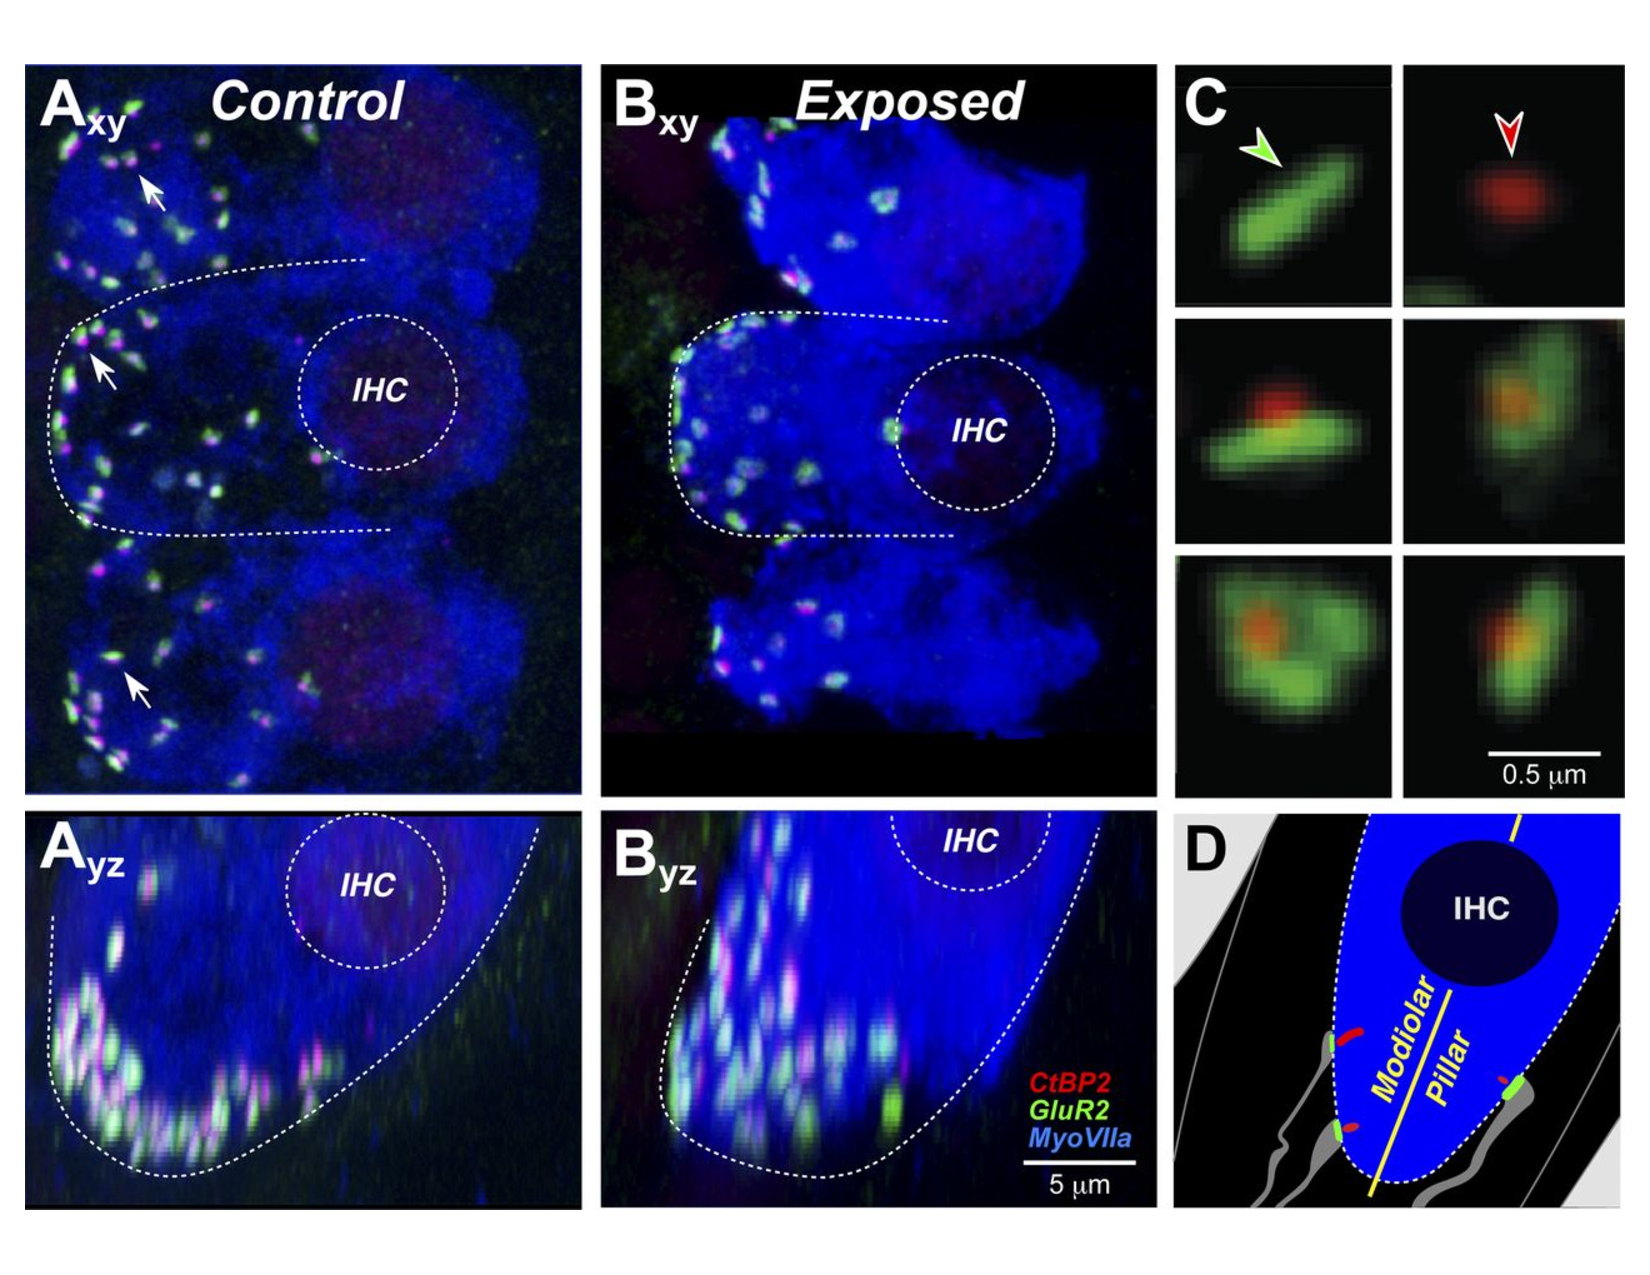
\includegraphics[width=0.95\textwidth]{furman-2.pdf}
	\caption[Deafferentation of Inner Hair Cells]{Deafferentiation of IHCs precedes hair cell death in noise exposed mice.  Figure is reprinted from~\cite{Furman2013NoiseInduced}.  Panels A  and B show a triple-stained cross sectional view of an IHC.  Synaptic ribbons are in red, and glutamate-receptor patches are in green; deafferentiation is visible when they are not paired (in C).  }
	\label{fig:furman-2}
\end{figure}


\cite{Sergeyenko2013AgeRelated} extended this work to demonstrate that this deafferentiation may also arise solely as a function of time.  In a study of mice aged 4 to 144 weeks that were never exposed to loud sounds, a similar loss of hair cell projections was observed.


\section{Physiology of the Auditory Nerve} % (fold)
\label{sec:physiology_of_the_auditory_nerve}
\subsection{Spontaneous Rates of Fibers} % (fold)
\label{sub:spontaneous_rates_of_fibers}
In the absence of stimulus, individual fibers of the auditory nerve exhibit a wide range of average firing rates: human AN fibers have spontaneous rates between 0--120 spikes/second.  Any individual fiber's spontaneous rate varies slowly over time, but will fall within a relatively narrow band.  The fibers of the auditory nerve are divided into two, or sometimes three, categories: low-, medium-, and high spontaneous rate (SR).  Different authors assign different maximum firing rates to each category:~\cite{Temchin2008Threshold} categorizes SRs below 18 spikes/second to be ``low/medium'', and anything above that to be ``high''.  Others, such as~\cite{Liberman1978AuditoryNerve}, define only two categories.  
% subsection spontaneous_rates_of_fibers (end)
\subsection{Low Spontaneous Rate Fibers Suffer Selective Losses} % (fold)
\label{sub:low_spontaneous_rate_fibers_suffer_selective_losses}
\cite{Furman2013NoiseInduced} and others have demonstrated that noise-induced cochlear synaptopathy is selective for low-SR fibers, particularly at high frequencies.  As shown in \autoref{fig:furman-5}, examination of fiber loss after acoustic trauma demonstrates a preferential loss of low-SR fibers, particularly above 4 kHz.  

\begin{figure}[htbp]
	\centering
	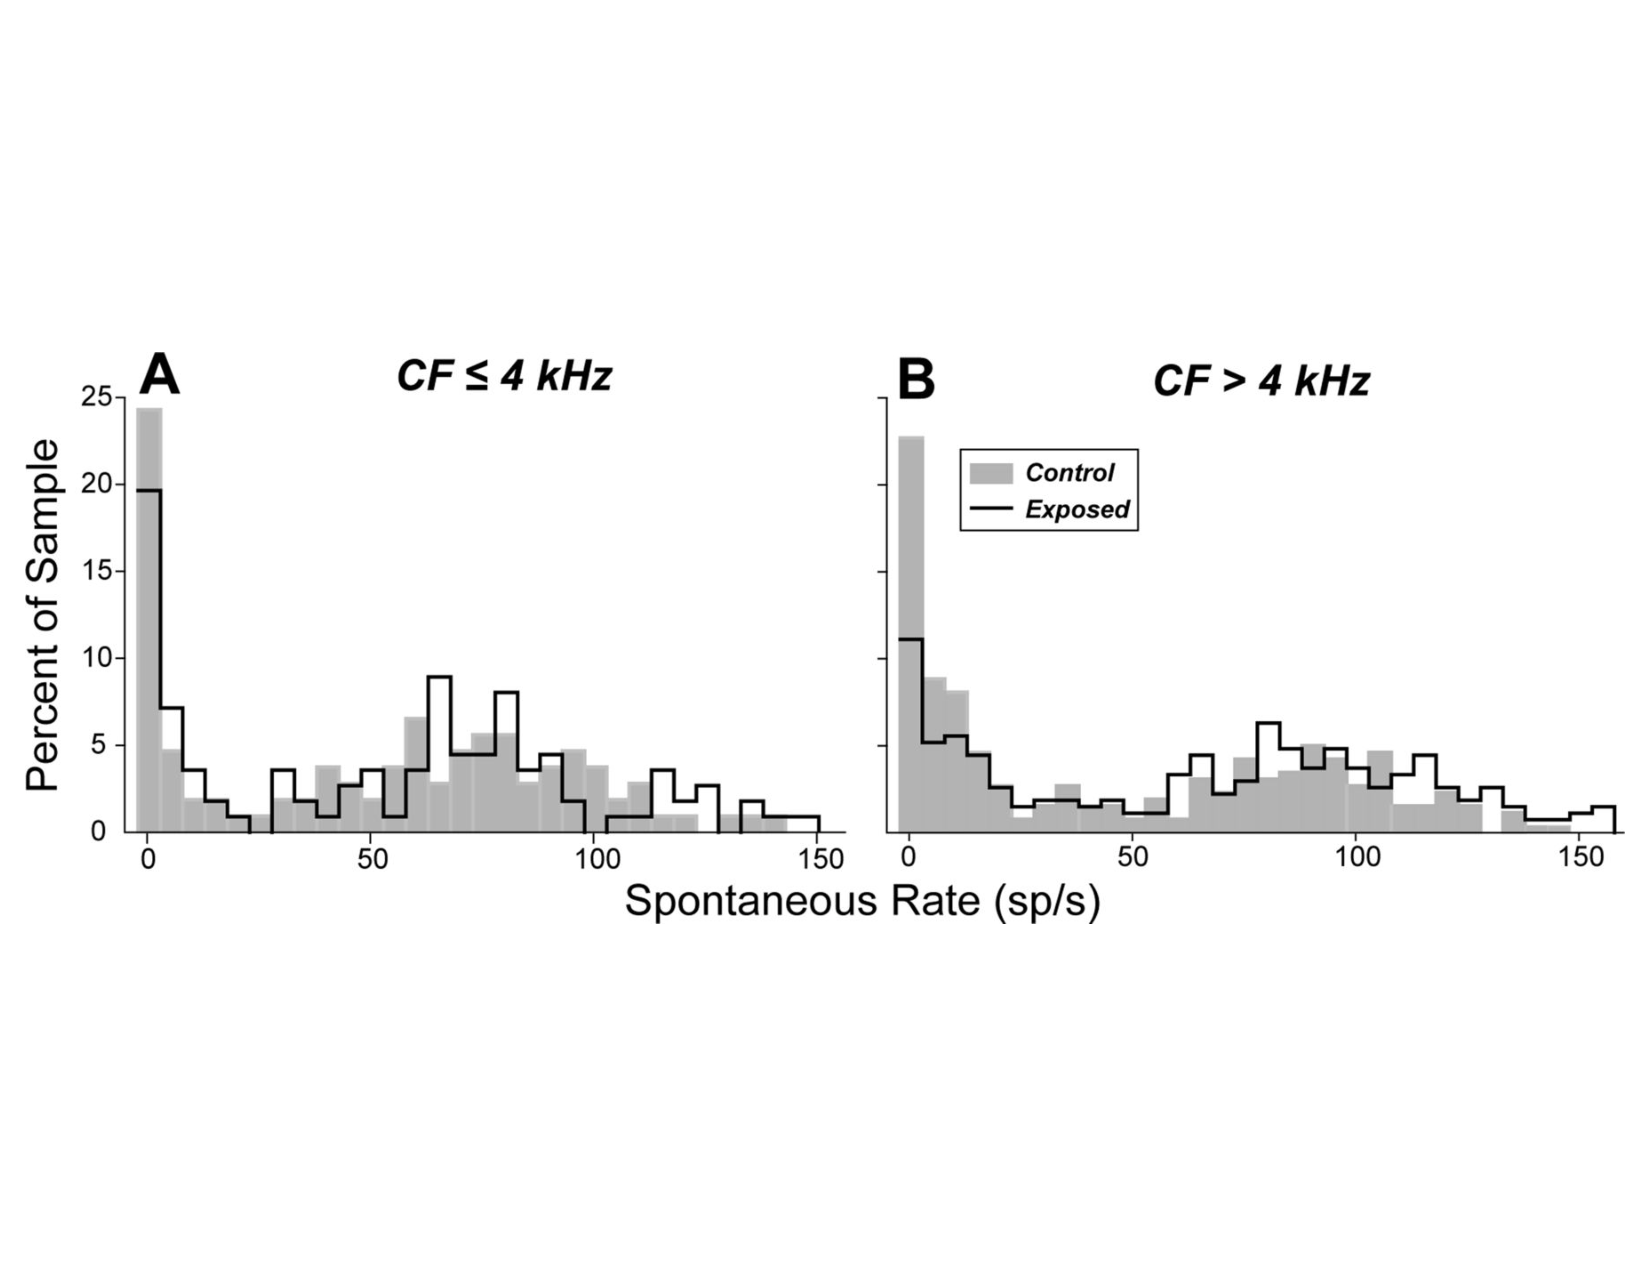
\includegraphics[width=0.95\textwidth]{furman-5.pdf}
	\caption[Synaptopathy is Selective]{Synaptopathy is selective for fibers with low spontaneous rates, and particularly selective for low-SR fibers at high frequencies. Figure reprinted from~\cite{Furman2013NoiseInduced}}
	\label{fig:furman-5}
\end{figure}

\subsection{Fiber SR Distribution is Not Tonotopically Uniform} % (fold)
\label{sub:fiber_rates_are_tonotopically_nonuniform}
Along the length of the basilar membrane, different percentages of low-, medium-, and high-SR fibers innervate each IHC.  \cite{Temchin2008Threshold,Temchin2014Spatial,Bourien2014Contribution} have demonstrated in chinchilla and mongolian gerbil that there is a nonlinear distribution of low-SR fibers along the basilar membrane, with significantly more low-SR fibers per IHC at high frequencies.   A distribution of fiber rates per CF is given in \autoref{fig:temchin-1}.

\begin{figure}[htbp]
	\centering
	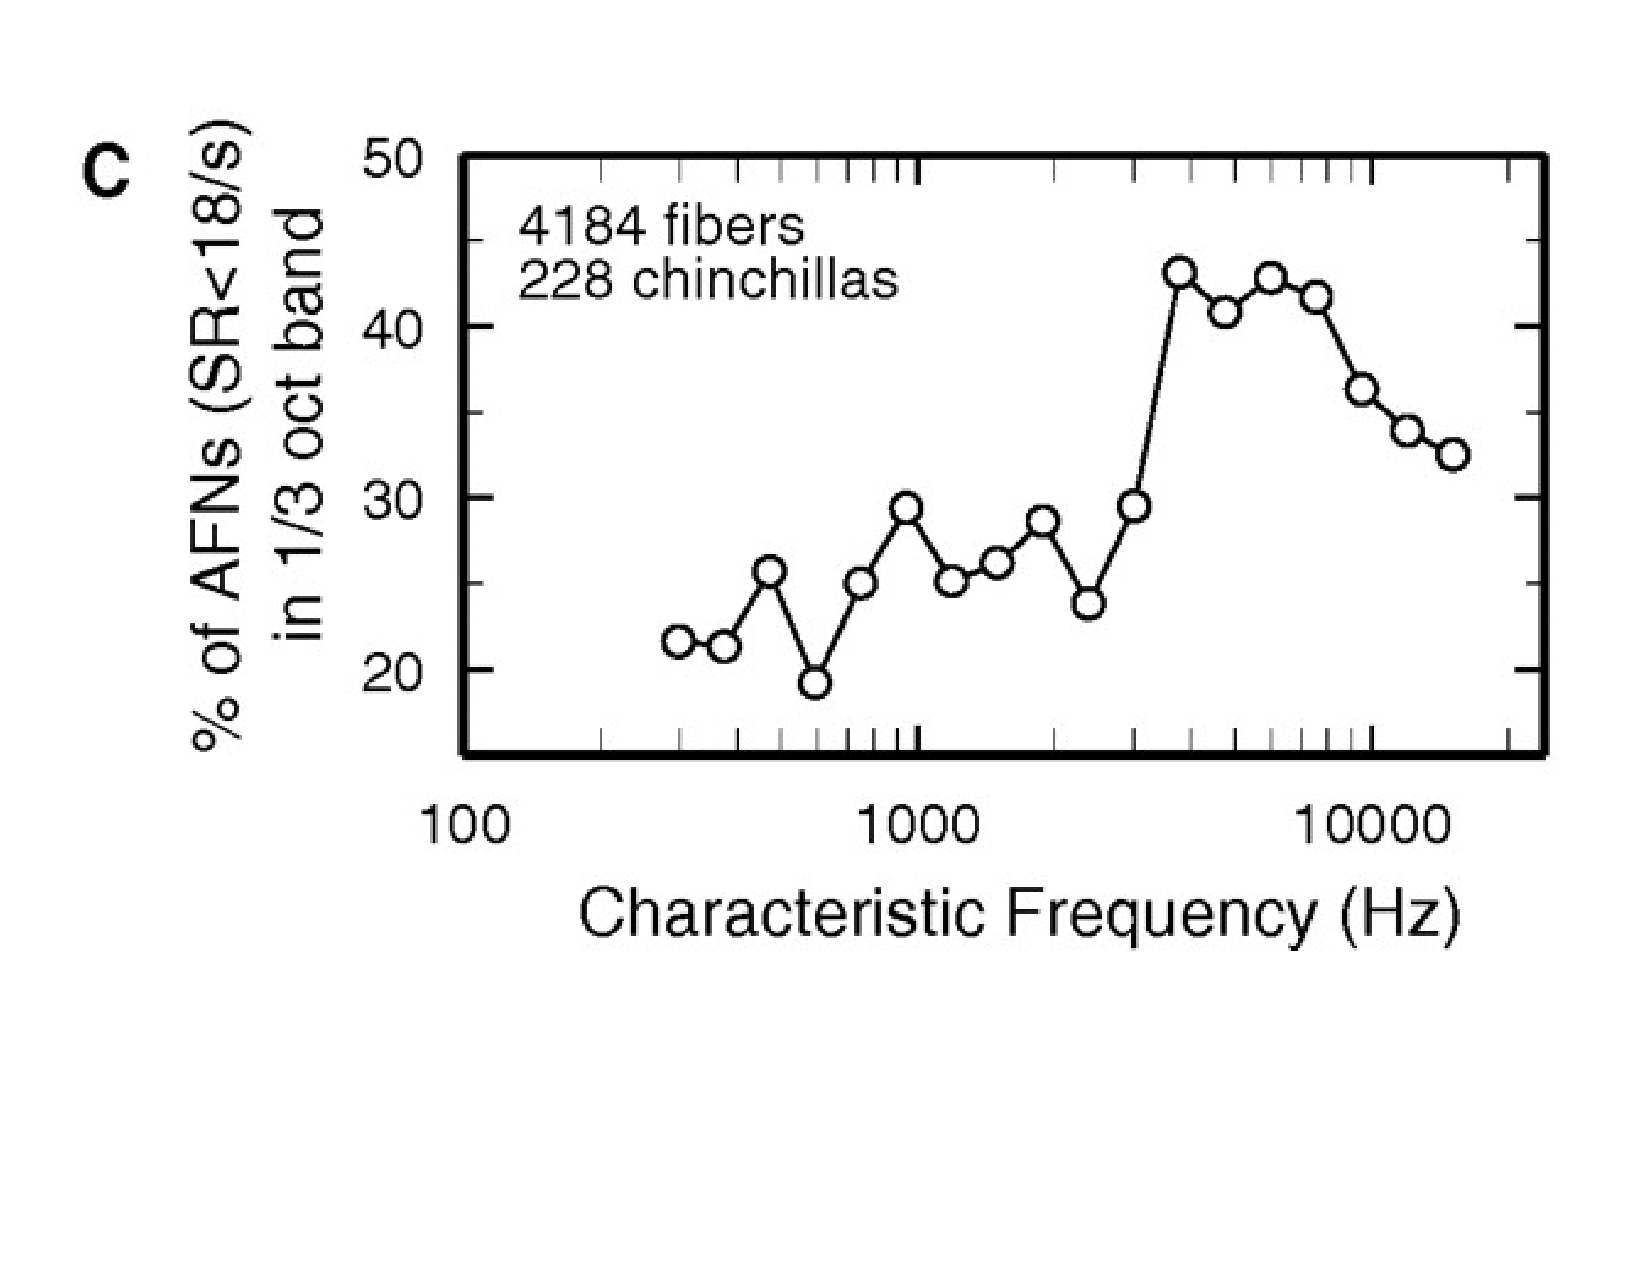
\includegraphics[width=0.95\textwidth]{temchin-1c.pdf}
	\caption[Distribution of Fiber Type]{Distribution of Fiber Type. Conventional extracellular recording electrodes characterized the spontaneous rate of 4184 individual AN fibers in 228 chinchilla along the length of the Organ of Corti. Reprinted from \cite{Temchin2008Threshold}}
	\label{fig:temchin-1}
\end{figure}
% subsection fiber_rates_are_tonotopically_nonuniform (end)

\section{Relevant Functional Neuroanatomy of the Auditory Midbrain} % (fold)
\label{sec:relevant_functional_neuroanatomy_of_the_auditory_midbrain}
Ascending from the AN, auditory information passes through multiple brainstem and midbrain areas en route to the thalmus, and then auditory cortex.  A simplified schematic of pre-thalamic connections is given in \autoref{fig:covey-1}. 

ABR Waves III and V are thought to reflect, in part, the synchronous contributions of the Cochlear Nucleus and Inferior Colliculus, it is important to consider both the effects of CS as well as more local physiology on the overall ABR.

\begin{figure}[htbp]
	\centering
	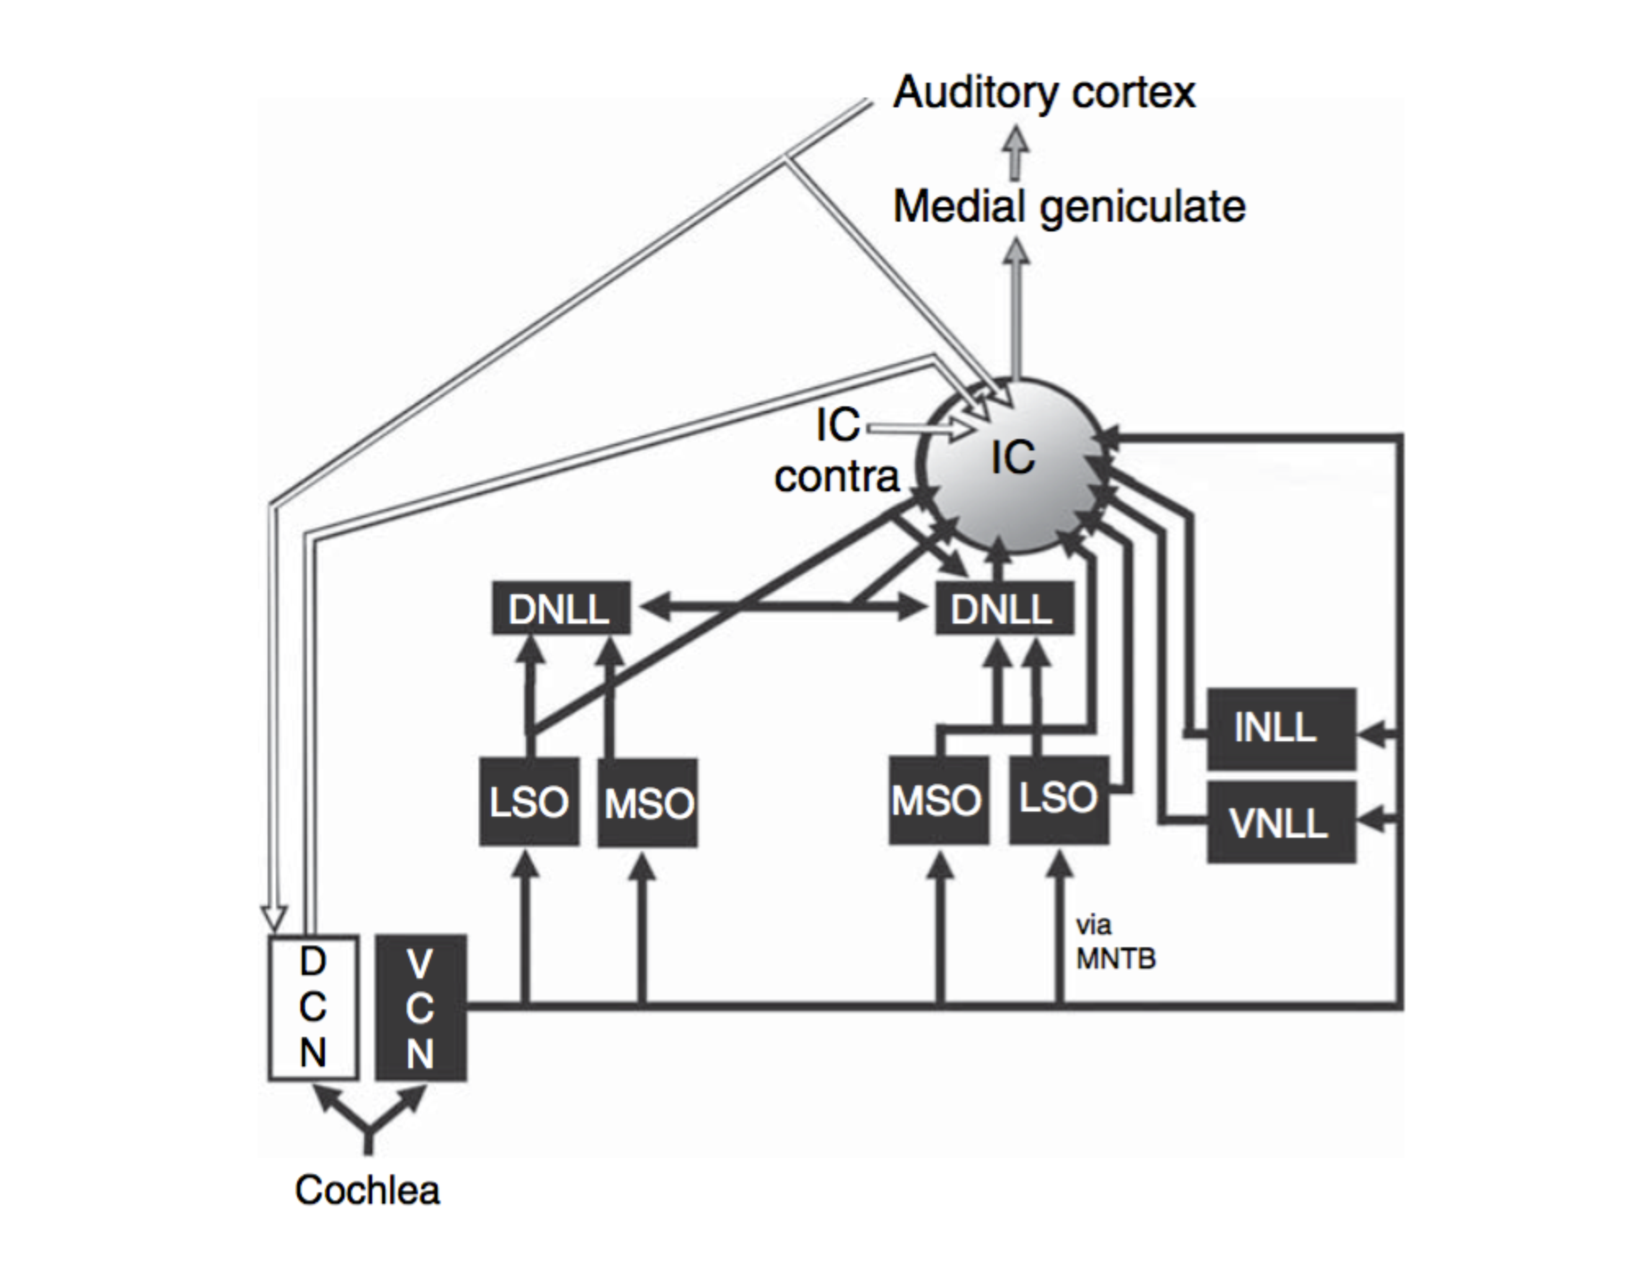
\includegraphics[width=0.95\textwidth]{covey-1.pdf}
	\caption[Ascending Auditory Pathway]{A simplified network diagram of the ascending auditory pathway in mammals.  Pathways in white arise from the DCN; pathways in black from the VCN.  Figure reprinted from \cite{Covey2008Inputs}.}
	\label{fig:covey-1}
\end{figure}

\subsection{The Cochlear Nucleus} % (fold)
\label{sub:the_cochlear_nucleus}
The primary projection from the AN is the Cochlear Nucleus, an inhomogenous structure that is the first auditory relay station located in the ipsilateral medulla of the brainstem.  
\subsection{The Dorsal Cochlear Nucleus} % (fold)
\label{sub:the_dorsal_cochlear_nucleus}
\cite{Ryugo2008Projections} demonstrated in cat that low-SR fibers have a anatomical projection bias towards the small cap of the Dorsal Cochlear Nucleus.  While low-SR fibers project to many areas, the small cap receives input from low-SR fibers exclusively, suggesting a selective role for low-SR projections. \cite{Liberman1993Central} found similar results. 

Further, while projections are selective as shown in \autoref{fig:ryugo}, the projections have relatively shallow but broad arbors. This anatomical specificity of projection combined with a breadth of coverage supports a particular role for low-SR fibers, and does not rule out the possibility of further specificities in higher brainstem and midbrain areas. 

\begin{figure}[htbp]
	\centering
	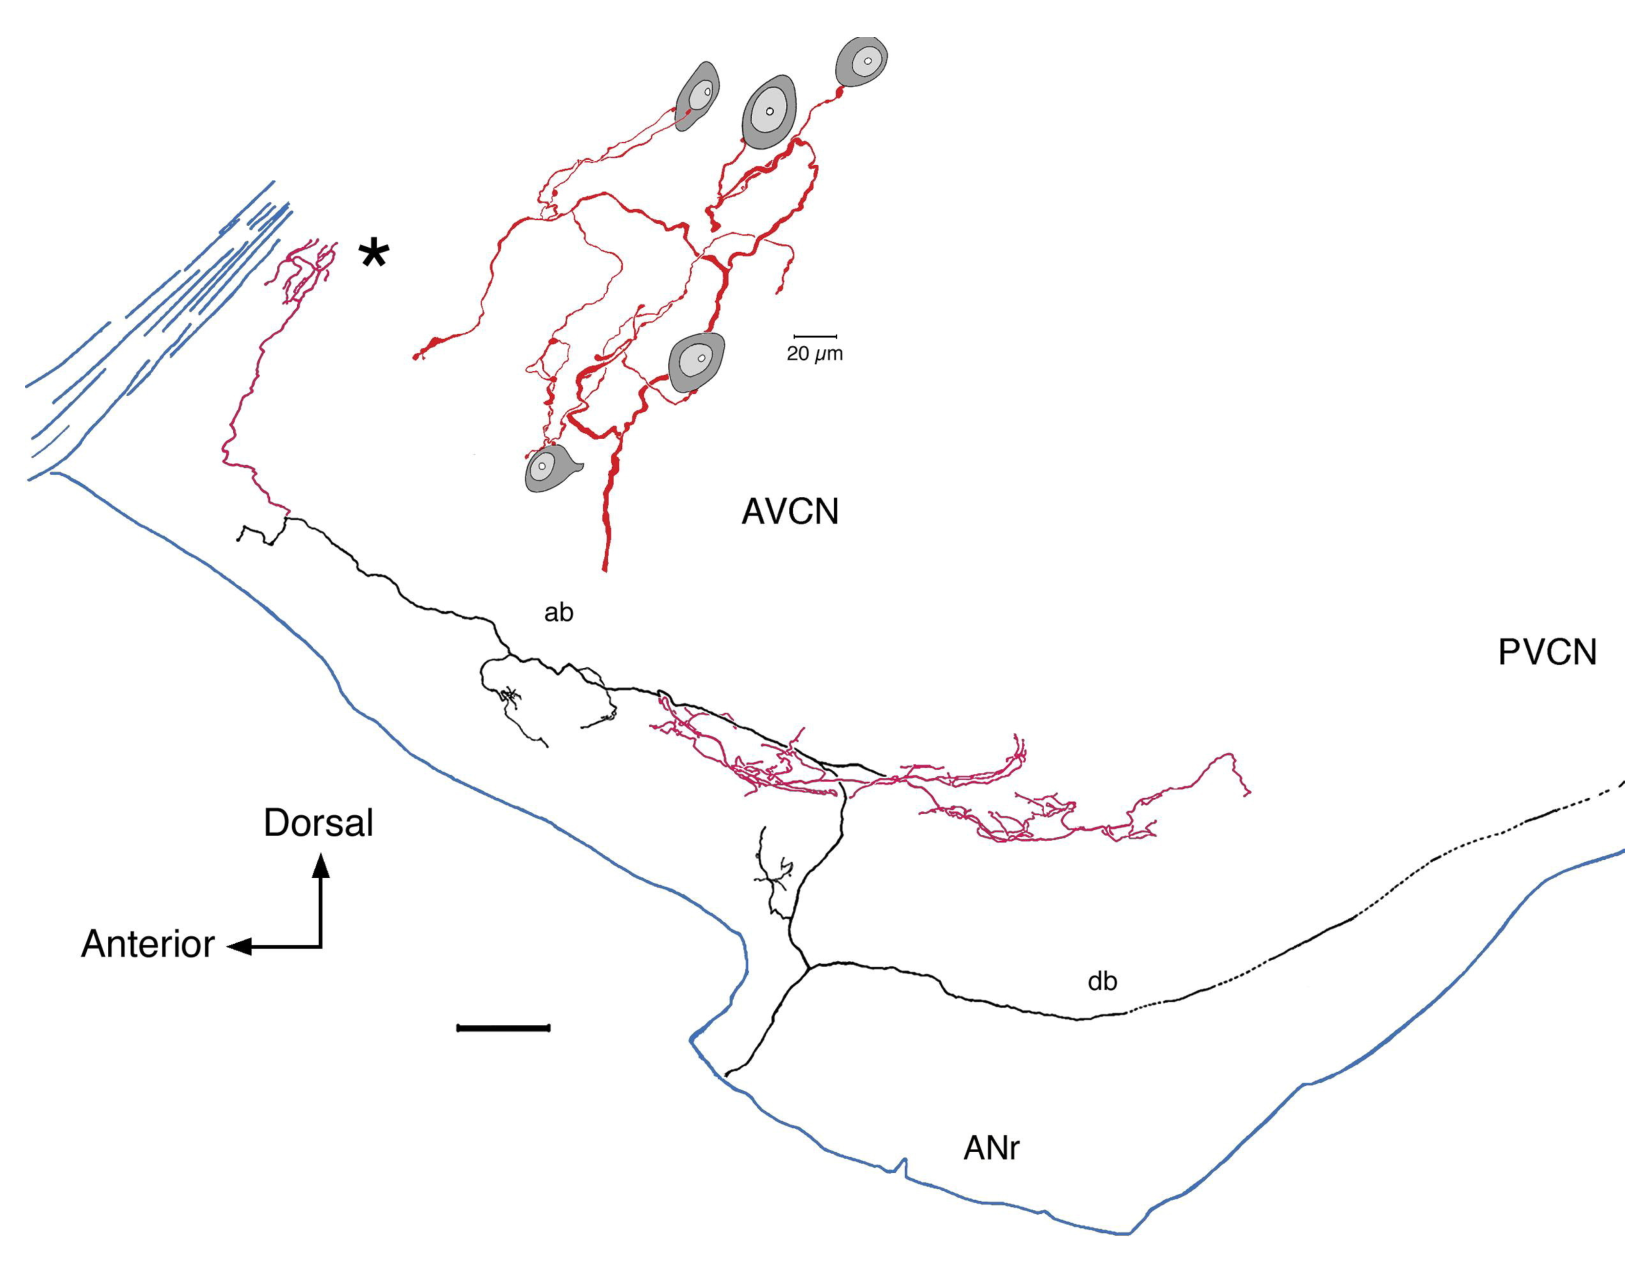
\includegraphics[width=0.95\textwidth]{ryugo-1.pdf}
	\caption[Low SR Fibers Project to the Small Cap]{Low-SR fibers project to the Small Cap area of the DCN.  From~\cite{Ryugo2008Projections}, this shows a lateral view of a low SR fiber as it collateralizes (red) in the rostral and lateral SCC (CF=0.45 kHz; SR=1.2 s/s; Th=34 dB SPL).}
	\label{fig:ryugo}
\end{figure}

While the VCN is critically important for the processing of binaural phenomena, the specificities of projection observed in the DCN suggest an interesting role for synaptopathic losses that may be more monaural.  Further, DCN projects directly to IC, wheras a proper consideration of contributions from the VCN would require a more involved treatment of pre-collicular regions such as the MSO. 
% subsection the_ventral_cochlear_nucleus (end)
\subsection{The Inferior Colliculus} % (fold)
\label{sub:the_inferior_colliculus}
The IC has long been regarded as the last pre-thalamic obligate waystation for ascending auditory information, and a major center of pre-cortical auditory processing with many diverse functions \citep{Cant2005Atlas,Covey2008Inputs,Moore1985Projections}.

Recently,~\cite{Beebe2016Extracellular} has reported at least four morphologically different GABAergic neural types in IC that react in different ways to auditory stimuli.  Considering the recent diversity of IC responses that have been observed and will be discussed in \autoref{sub:the_carney_model}, this is a tantalizing anatomical observation that may correlate with electrophysiologically observed behavior.  


% subsection the_inferior_colliculus (end)
% section functional_neuroanatomy_of_the_auditory_midbrain (end)

\section{Models of the Auditory Periphery} % (fold)
\label{sec:models_of_the_auditory_periphery}
\subsection{The Verhulst Model} % (fold)
\label{sub:the_verhulst_model}
A functional model of the auditory periphery was developed by~\cite{Verhulst2015Functional}.  As outlined in \autoref{fig:verhulst-1}, the model consists of a middle ear preprocessing model adapted from~\cite{Meddis2010Computational}.  Input is passed to a cochlear transmission line model, which estimates BM displacements and velocities for an arbitrary number of BM sections (default: 1000).  Motions of the BM are translated into IHC bundle deflections and passed through a nonlinearity.  Estimates of the Instantaneous Firing Rate (IFR) are made by a method adapted from~\cite{Westerman1988Diffusion}, which implements a three-store diffusion model of synaptic vesicle and neurotransmitter release and reuptake.  Unlike the Zilany model, the Verhulst model does not account for per-fiber noise in spontaneous rate.

The version of the model given by~\cite{Verhulst2015Functional} also includes a CN and IC modeling stage from~\cite{Nelson2004Phenomenological}, and the final model output are estimates of ABR Wave I, Wave III, and Wave V. 

\begin{figure}[htbp]
	\centering
	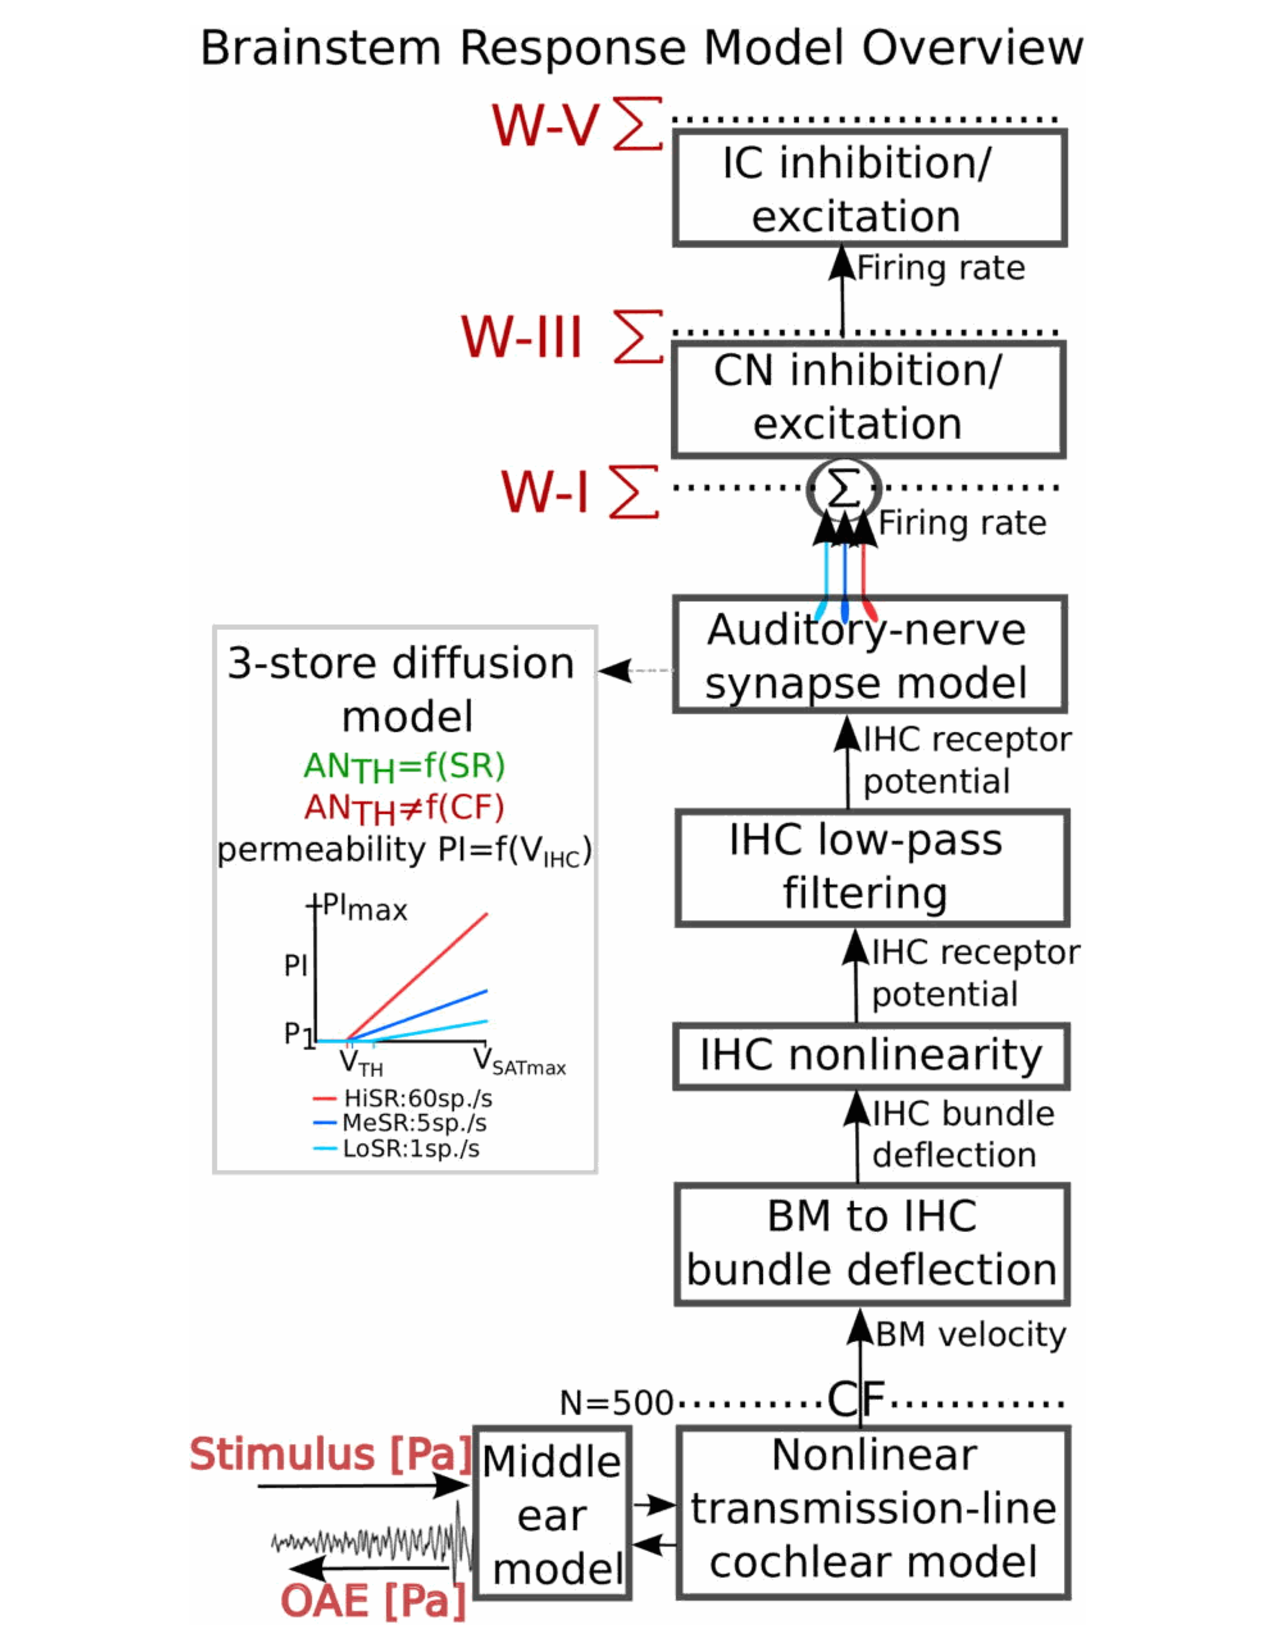
\includegraphics[width=0.95\textwidth]{verhulst-1.pdf}
	\caption[The Verhulst Model]{Major subunits of the Verhulst transmission line model of the auditory periphery.  Figure is reprinted from~\cite{Verhulst2015Functional}.  Input (stimulus) and outputs (OAEs, Wave I, Wave III, Wave V) are in red, and located at their physiologically relevant leves.}
	\label{fig:verhulst-1}
\end{figure}


\subsection{The Zilany and Bruce Model} % (fold)
\label{sub:the_zilany_and_bruce_model}
\cite{Zilany2006Modeling} proposed a phenomenological, signals-driven model of the auditory periphery.  It has been refined and updated since to account for an increasing number of phenomena including estimations of speech intelligibility \citep{Zilany2007Predictions}, long-term IHC adaptation with power-law dynamics \citep{Zilany2009Phenomenological}, and updates to more closely model human parameters \citep{Zilany2014Updated}.  

The approach is outlined in \autoref{fig:zilany-1} and consists of a phenomenological power-law model that has filters for each stage of the periphery.  Fractional Gaussian noise is optionally added per-channel to simulate the stochasticities inherent in AN fiber spontaneous rates. 

\begin{figure}[htbp]
	\centering
	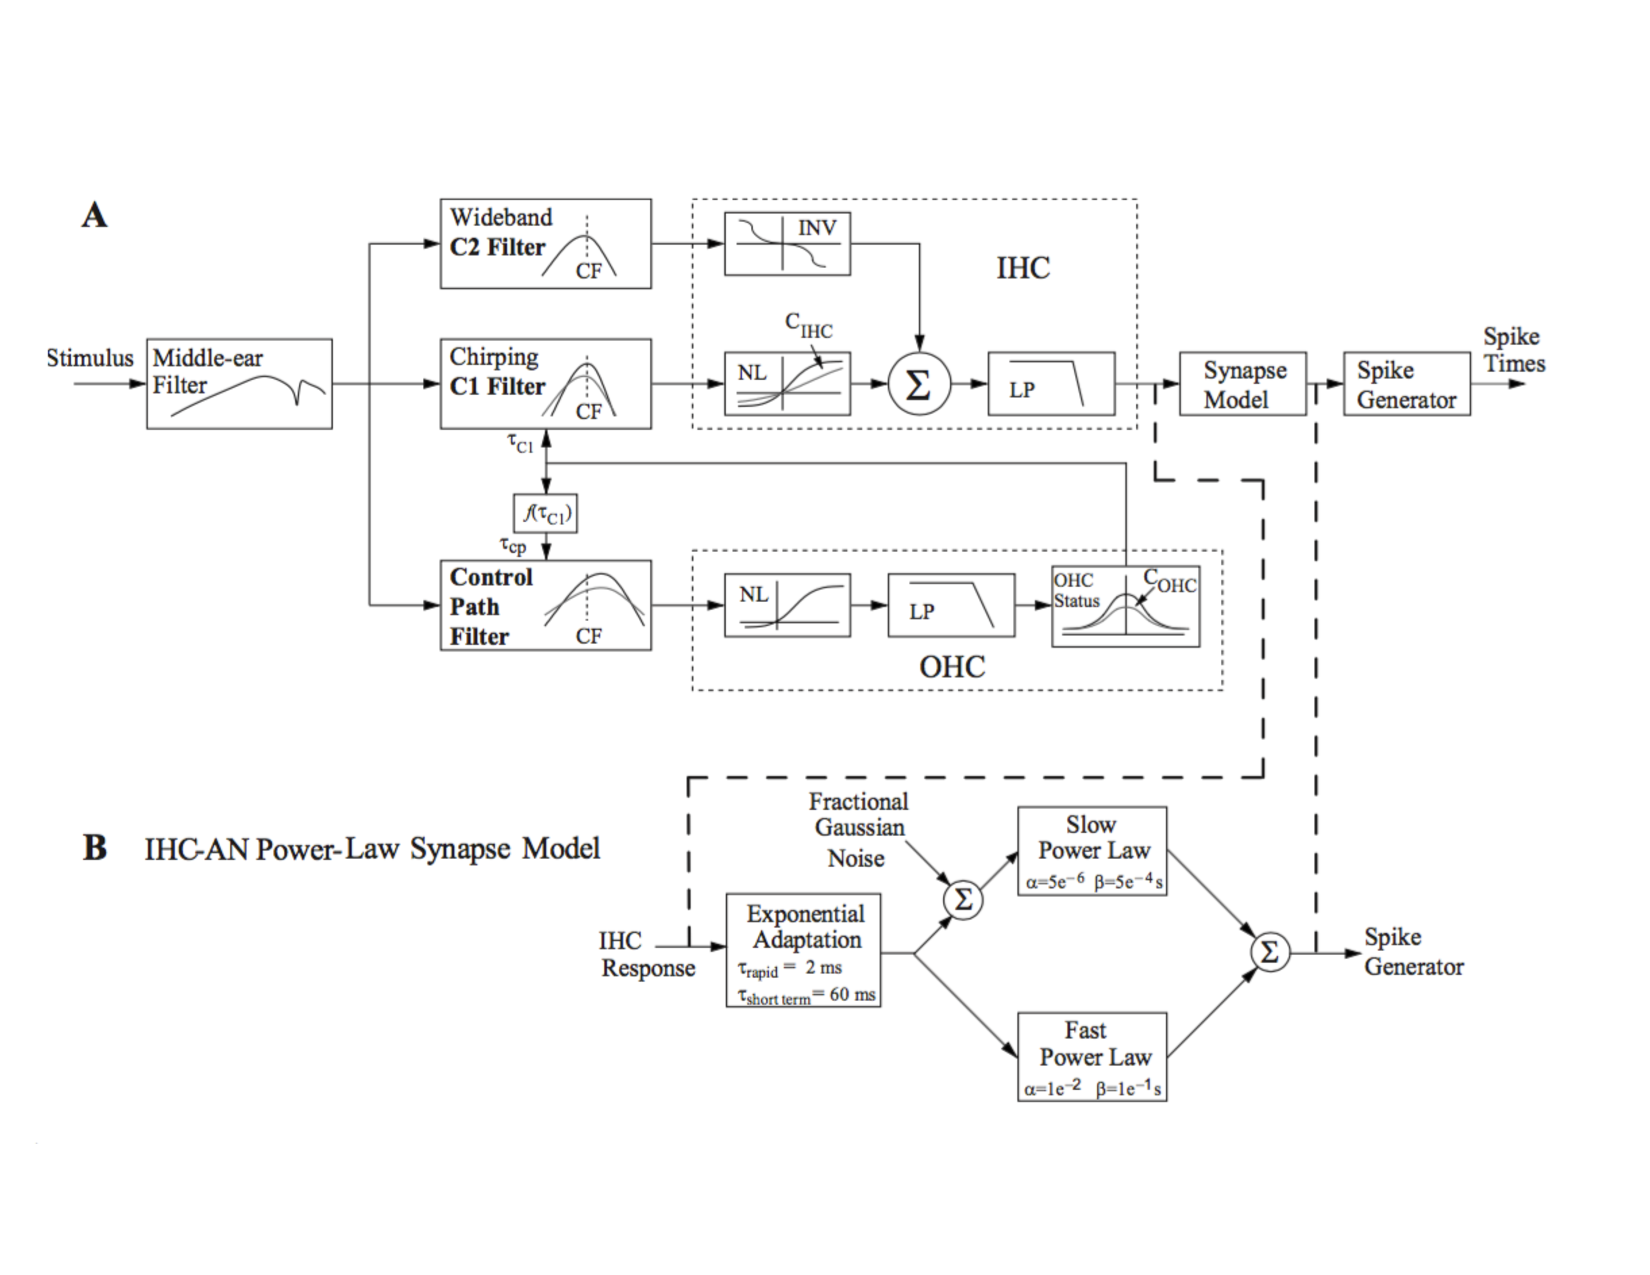
\includegraphics[width=0.95\textwidth]{zilany-1.pdf}
	\caption[The Zilany Model]{Major components of the Zilany model of the auditory periphery.  Figure reprinted from~\cite{Zilany2009Phenomenological}}
	\label{fig:zilany-1}
\end{figure}
% subsection the_zilany_and_bruce_model (end)
\section{Models of the Auditory Midbrain and Brainstem} % (fold)
\label{sec:models_of_the_auditory_midbrain_and_brainstem}
\subsection{The Nelson-Carney Model} % (fold)
\label{sub:the_nelson_carney_model}
\cite{Nelson2004Phenomenological} proposed a two-stage phenomenological model of the midbrain and brainstem.  The Cochlear Nucleus and Inferior Colliculus are each represented by a single Same-Frequency Inhibition Excitation (SFIE) filter, which convolves the output of the previous stage with  excitatory and inhibitory alpha functions.  As shown in \autoref{fig:nelsoncarney-1}, these functions' delays, amplitudes, and onset times can be adjusted to provide a tuned response for a given unit, compared to electrophysiological measurements.  In each case, each unit acts as a band-pass filter tuned to a certain bandwidth. 
\begin{figure}[htbp]
	\centering
	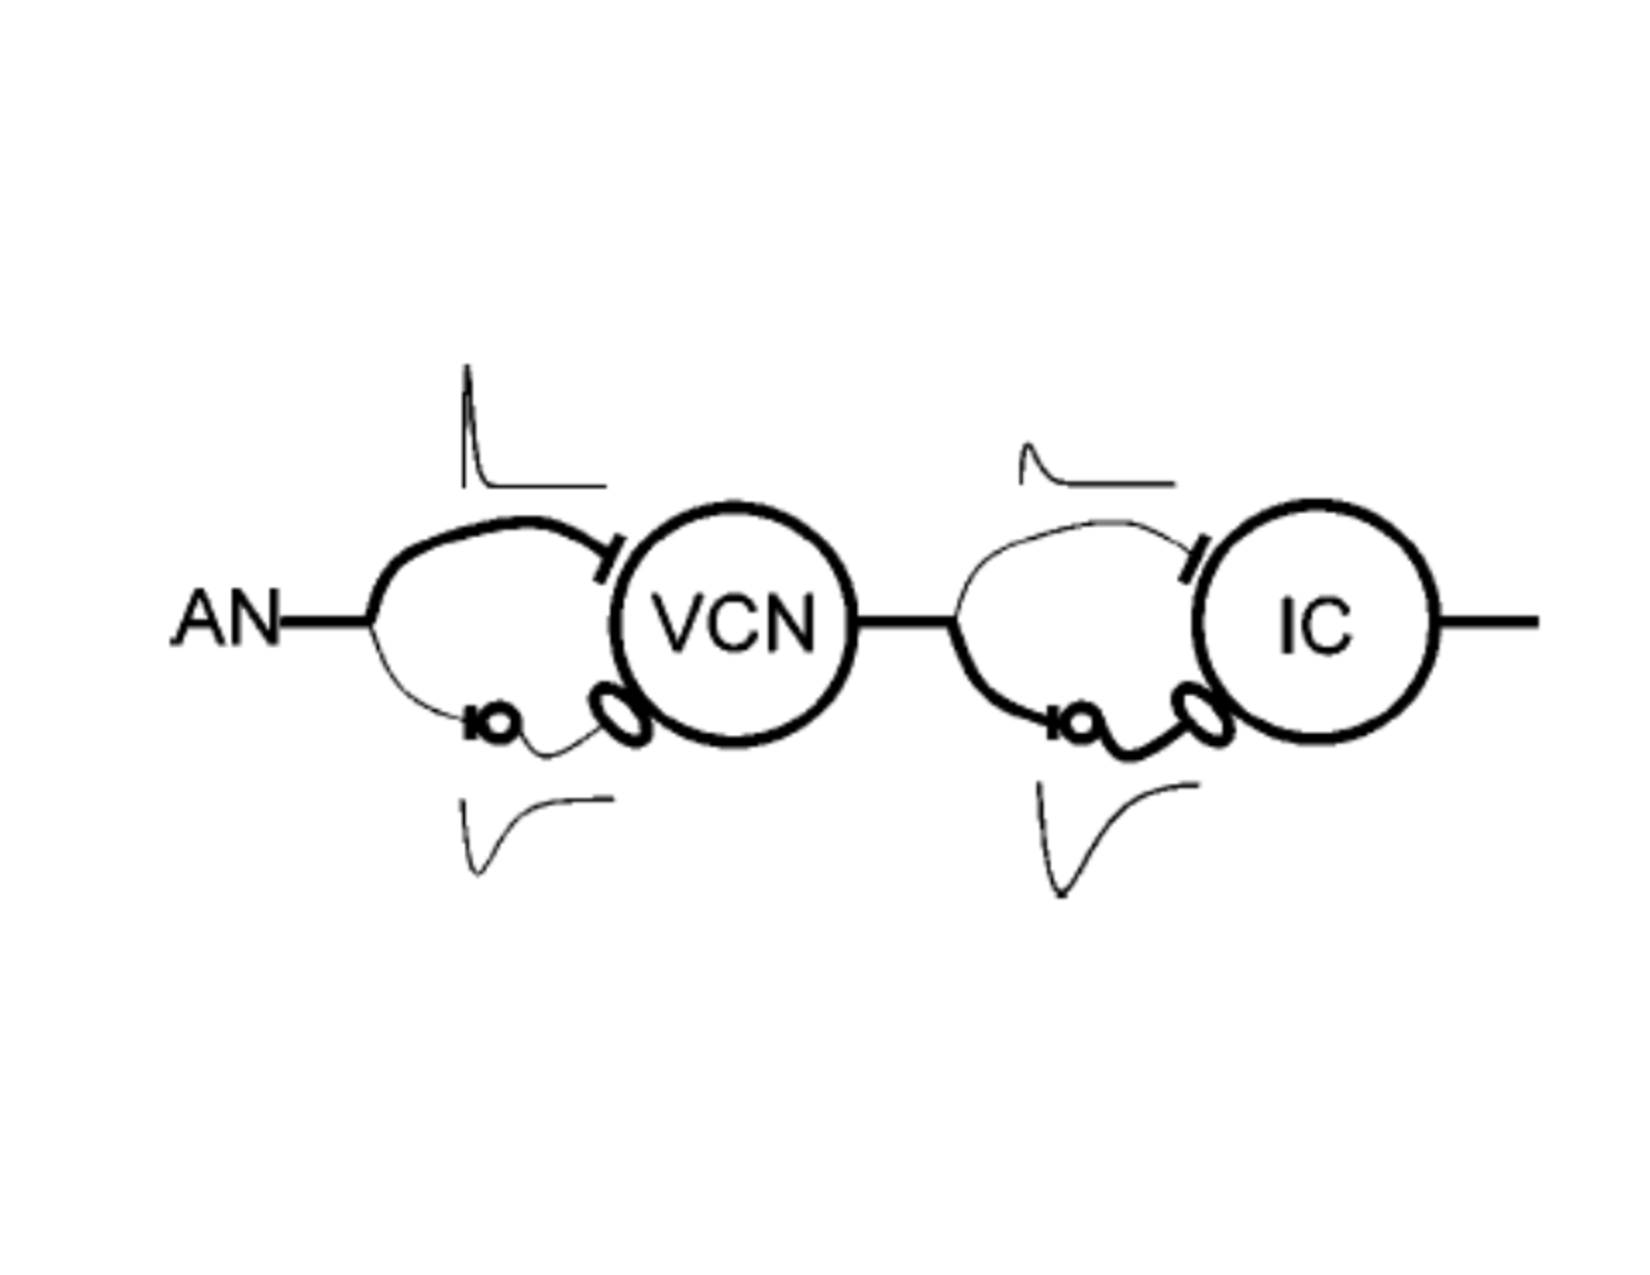
\includegraphics[width=0.95\textwidth]{nelsoncarney-1.pdf}
	\caption[The Nelson and Carney Model]{The Nelson and Carney Brainstem. Figure reprinted from~\cite{Nelson2004Phenomenological}.}
	\label{fig:nelsoncarney-1}
\end{figure}

\subsection{The Carney Model} % (fold)
\label{sub:the_carney_model}
\cite{Carney2015Speech} extended the two-stage \citeauthor{Nelson2004Phenomenological} model by the incorporation of three categories of IC responses, compared with the single filter in \autoref{sub:the_nelson_carney_model}, to better account for processing of spectrally complex vowel tones.  As shown in \autoref{fig:carney-1}, the IC is divided into three Same-Frequency Inhibition Excitation stages. 
\begin{figure}[htbp]
	\centering
	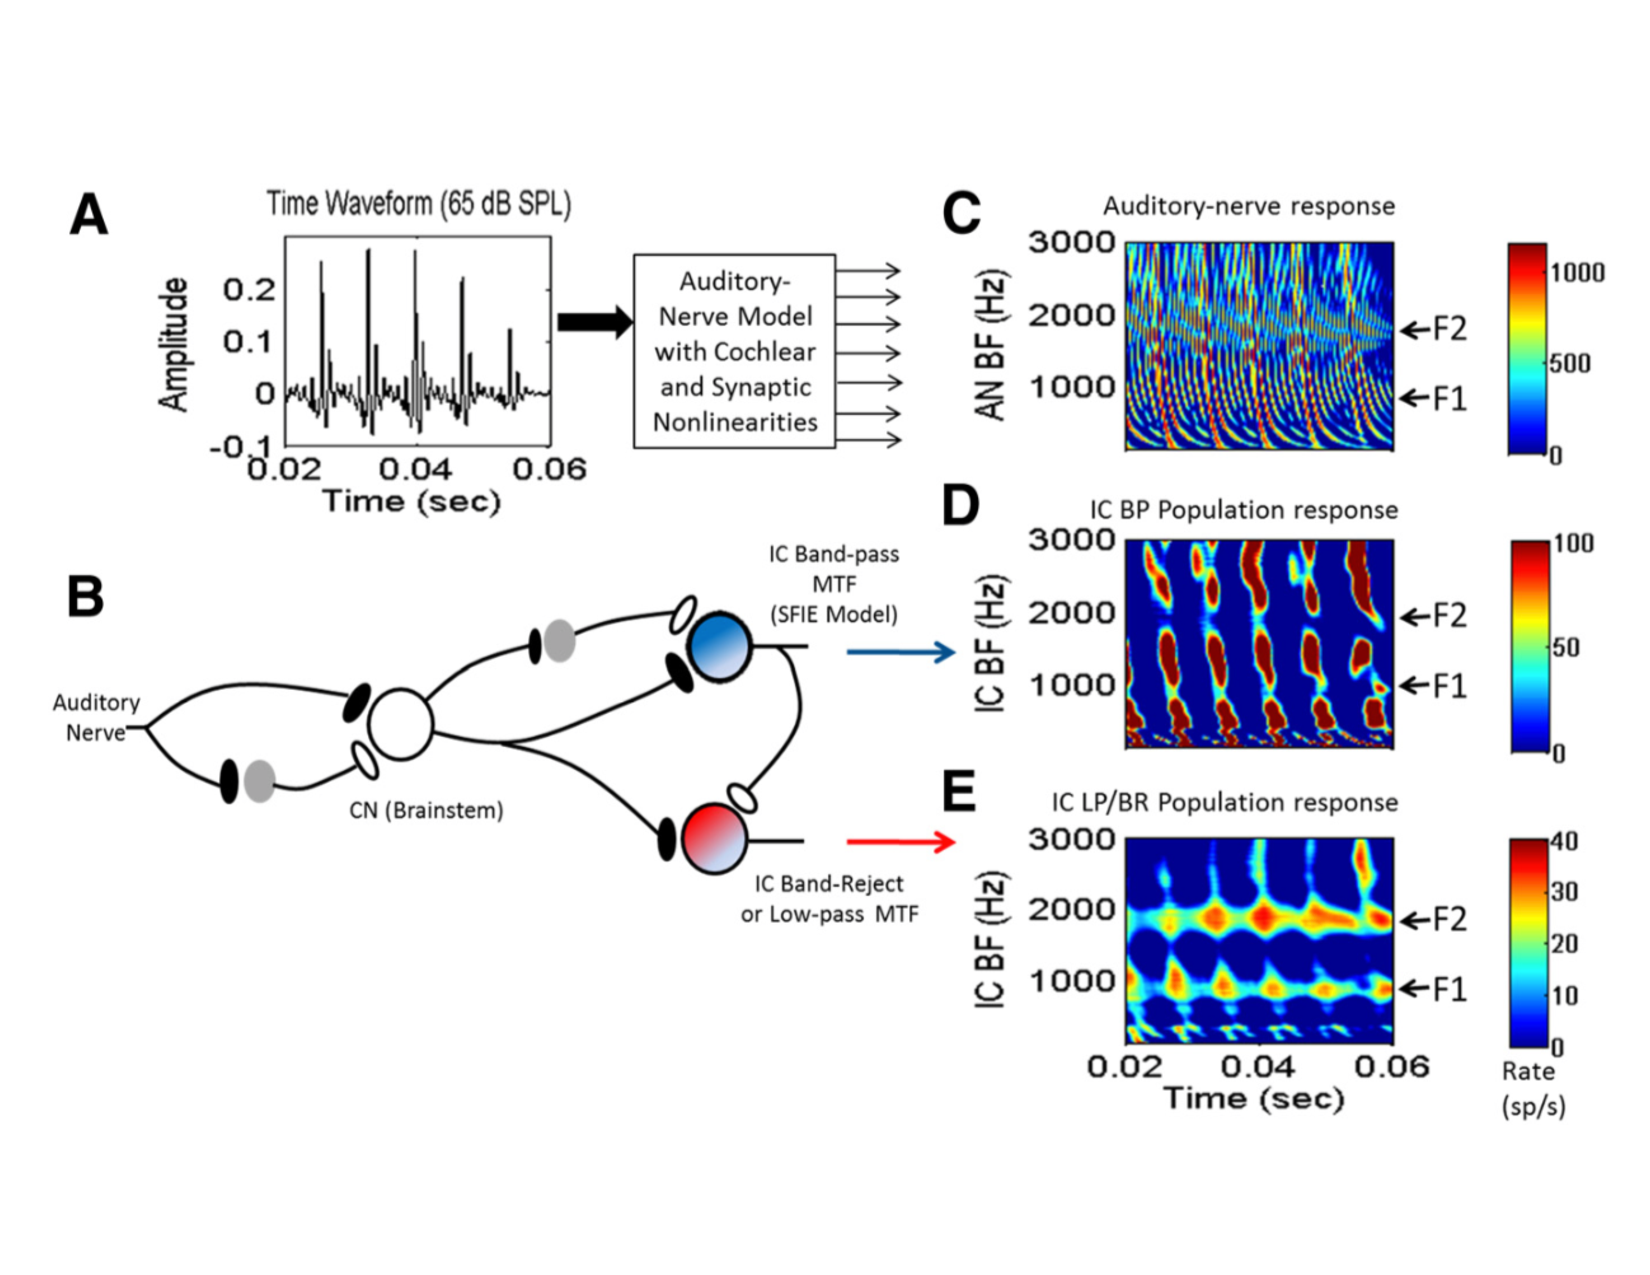
\includegraphics[width=0.95\textwidth]{carney-1.pdf}
	\caption[The Carney 2015 Model]{The Carney (2015) Midbrain and Brainstem.  Figure reprinted from~\cite{Carney2015Speech}}
	\label{fig:carney-1}
\end{figure}


Based on electrophysiological recordings in awake rabbits, \autoref{fig:carney-2} shows that \citeauthor{Carney2015Speech} represent 50\% of the IC as band-pass responses, 25\% as low-pass, and 25\% as band reject filters.  The weights were assigned based on the frequency of representation in IC.  

This three-stage IC model more fully accounts for the neural diversities that have been observed anatomically by \cite{Beebe2016Extracellular}, and is robust at high sound level and at background noise levels. 

\begin{figure}[htbp]
	\centering
	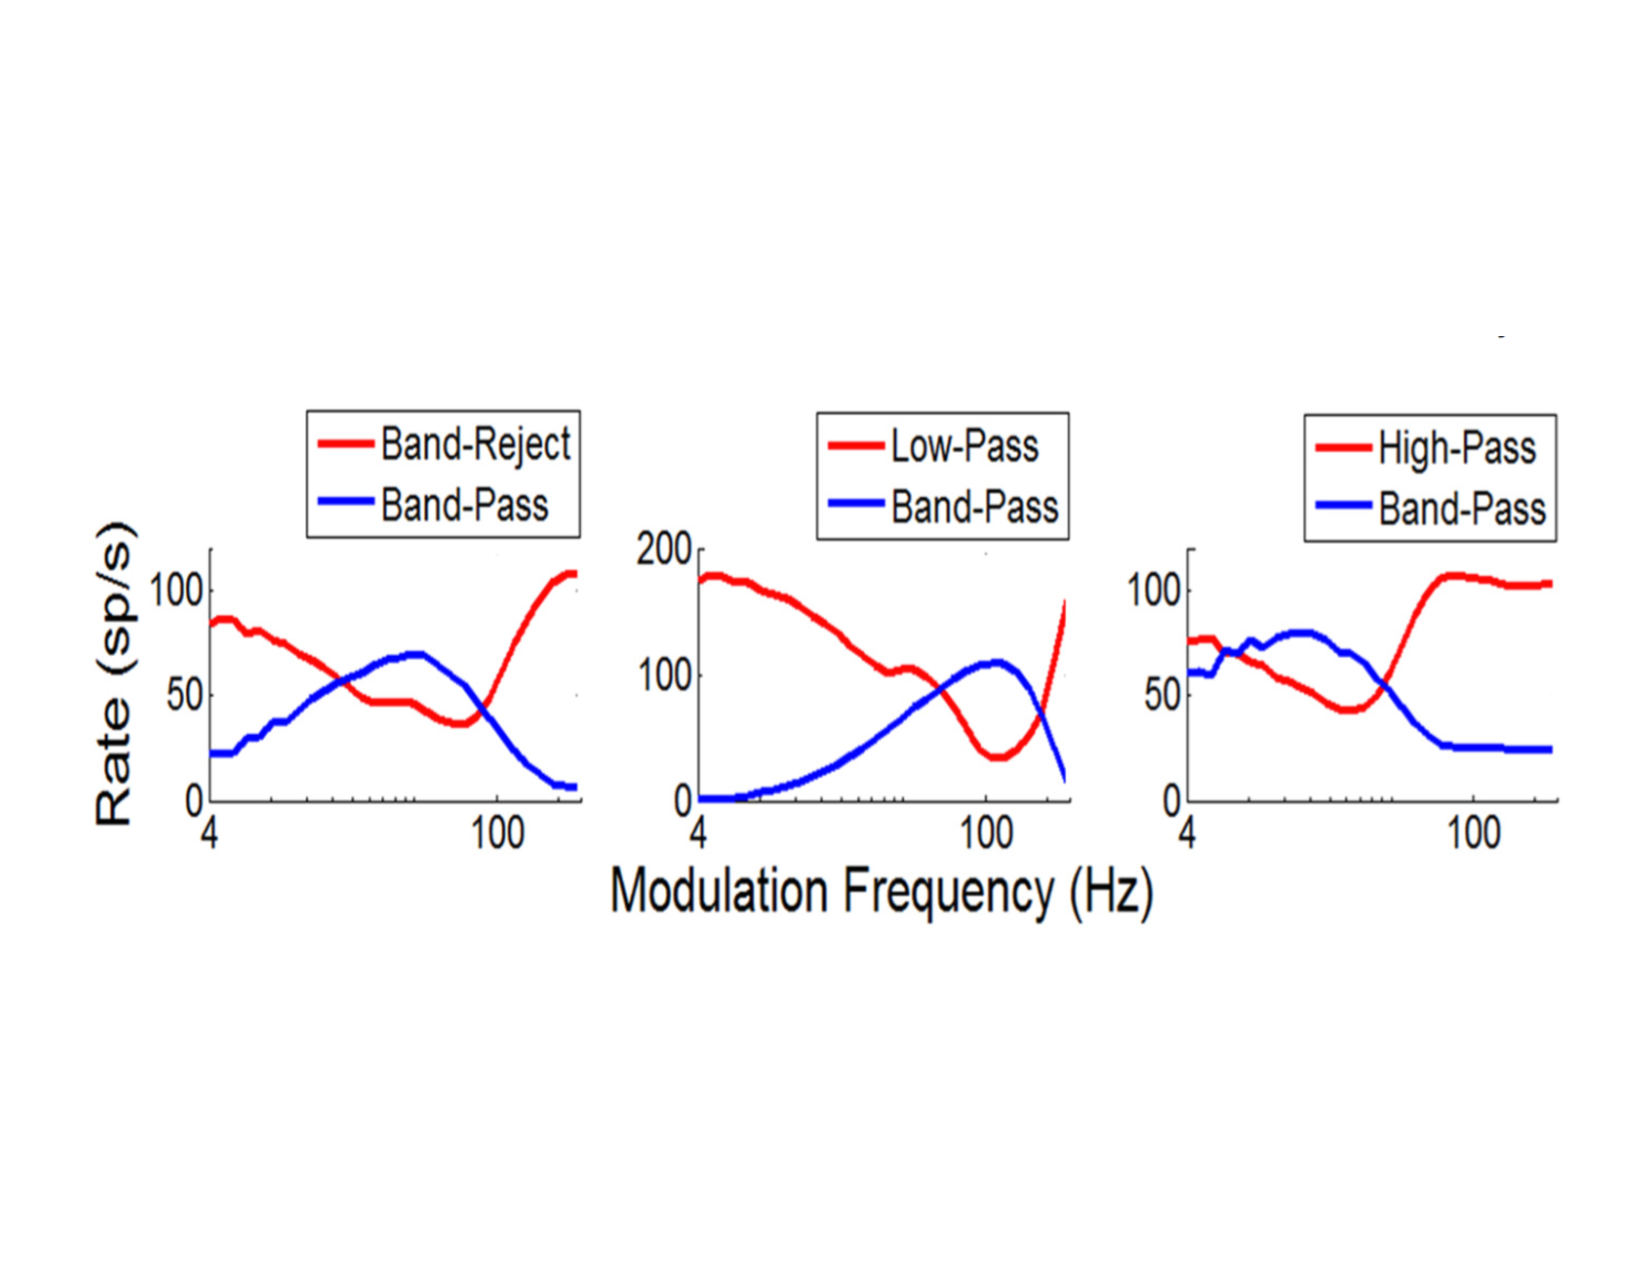
\includegraphics[width=0.95\textwidth]{carney-2.pdf}
	\caption[IC Response Types]{Different Response Types in the Carney Model.  Figure reprinted from~\cite{Carney2015Speech}}
	\label{fig:carney-2}
\end{figure}

\section{Candidate Objective Measures of Cochlear Synaptopathy in Humans} % (fold)
\label{sec:objective_measures_of_cochlear_synaptopathy}
To date, there is no objective test in humans that would give definitive insight into whether or not a patient exhibits signs of HHL, or be able to quantify the degree or location of impairment. 

\cite{Mehraei2015Auditory}, in an attempt to direct the search for such a diagnostic, correlated performance in a psychophysical task with markers in ABR.  In their work, 23 NHT listeners participated in a series of experiments to establish a relationship between task performance and putative cochlear synaptopathy.   Cochlear mechanics function was validated with click-evoked OAEs.  A behavioral measure of temporal sensitivity was established with an ITD envelope detection task with transposed tones.  Noise-masked ABRs were measured with increasing noise level.   As shown in \autoref{fig:mehraei-1}, Wave V latencies in increasing noise correlate with performance on ITD detection.

\begin{figure}[htbp]
	\centering
	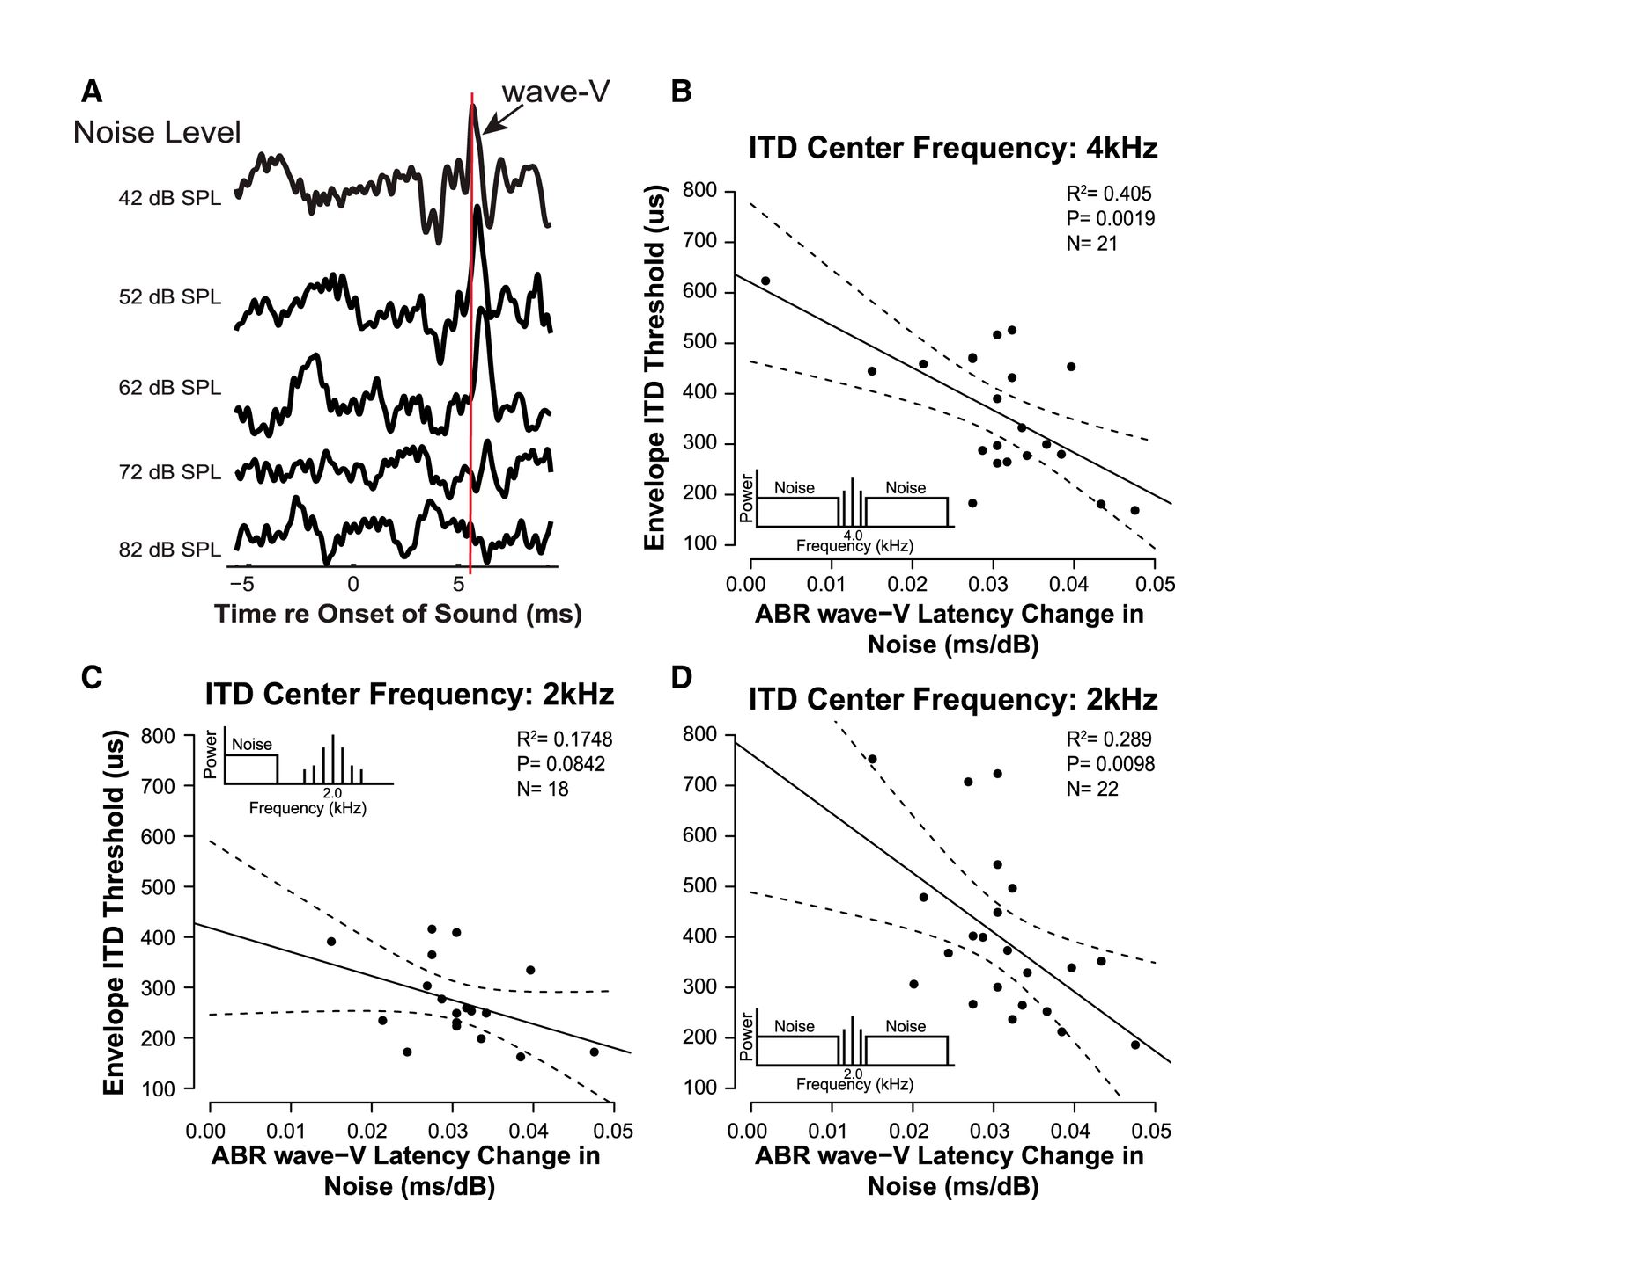
\includegraphics[width=0.95\textwidth]{mehraei-1.pdf}
	\caption[Wave V latency in noise]{Wave V latencies in increasing noise correlate with performance on ITD detection.  Figure reprinted from \cite{Mehraei2016Auditory}.}
	\label{fig:mehraei-1}
\end{figure}

It is hypothesized that the combination of high sound levels used and broadband noise maskers for ABRs both preferentially drive low-SR fibers and recruit their resistance to background noise.  Therefore, a synaptopathic-mediated decrease in low-SR fiber contributions would drive \emph{down} the latency shifts observed.
% section objective_measures_of_cochlear_synaptopathy (end)
